\documentclass{article}
\usepackage{palatino}
\usepackage{graphicx}
\usepackage[colorlinks=true]{hyperref}
\begin{document}

\section{The Story So Far}
We have a data visualization problem.
We can build the ``big picture'' of a project using a lattice representation, but:
\begin{itemize}
\item
  It is very hard to see high-cost regions at a glance.
\item
  The horizontal positioning of modules in the lattice carries no information.
\end{itemize}

Heat maps help estimate the overall cost of adding types, but still fix a horizontal ordering on modules.

We also have a scalability problem.
Whatever visual representation we choose should be reproducible for a project with 20 or 50 modules.
It should also scale to micro-level gradual typing.


\section{Proposal: Boxplots \& Violin Plots}
The lattice gets one thing very right, regardless of project size: it shows a clear progression from fully-untyped to fully-typed programs.
Boxplots carry this same message and tell about the distribution of running times.

\subsubsection*{Pros}
\begin{itemize}
\item
  Clear message: adding types step-by-step
\item
  Showcase the best, worst, average, and median for each level of types.
  The distribution is very easy to see.
\item
  Show less data overall, no extraneous details.
\item
  Boxplots are fairly easy to reproduce with low, constant-factor sampling
\end{itemize}


\subsubsection*{Cons}
\begin{itemize}
\item
  Configurations are not directly associated with runtimes
\item
  The number of data points for each box is not shown (or standard)
\item
  Some paths from left to right are invalid, but a boxplot does not show this.
\end{itemize}
We think the first point is a minor issue.
The second should be corrected; perhaps with a label, or by standardizing the counts across all levels.
We address the third by overlaying the least-sum path from fully-untyped to fully-typed.
This path shows the best way to move up the lattice while minimizing the runtime at each level.
It often spikes above the best minimum, showing that there is no royal road to gradual typing.


\section{Gallery}
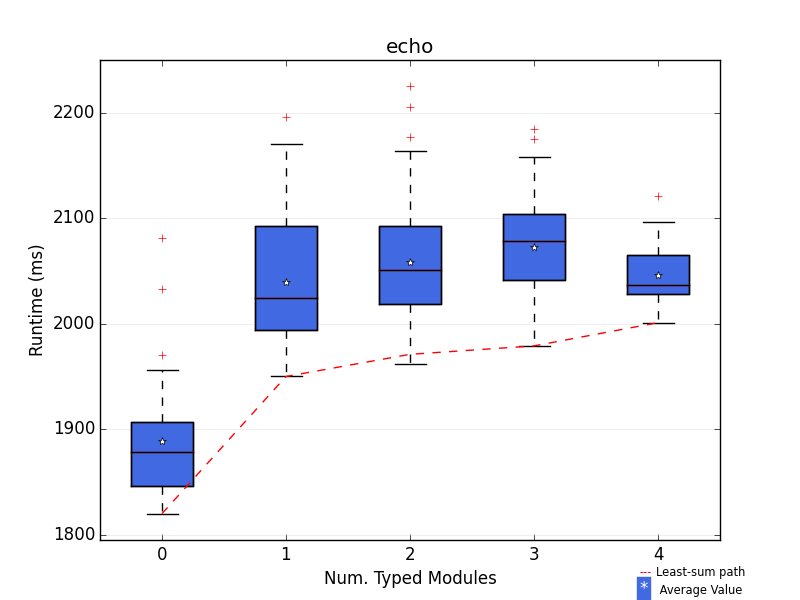
\includegraphics[width=\textwidth]{boxplots/echo-boxplot.png}
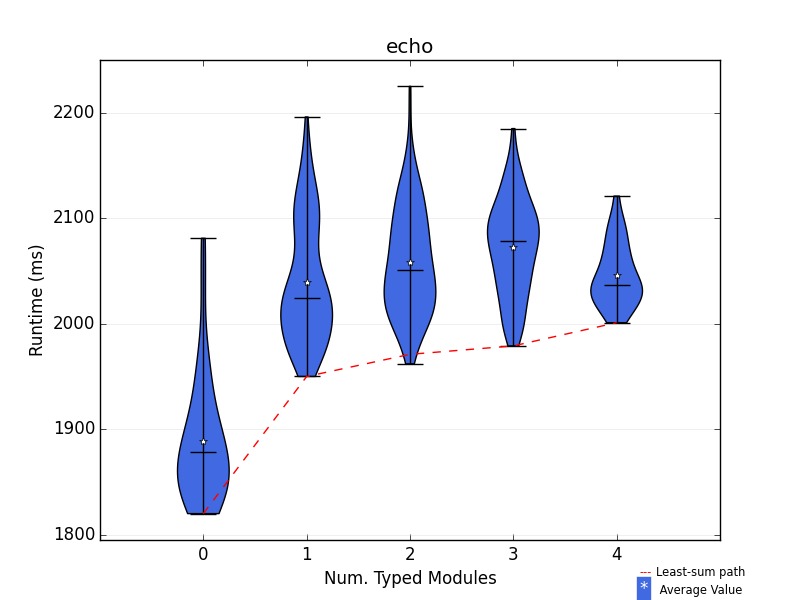
\includegraphics[width=\textwidth]{violins/echo-violin.png}
\newpage
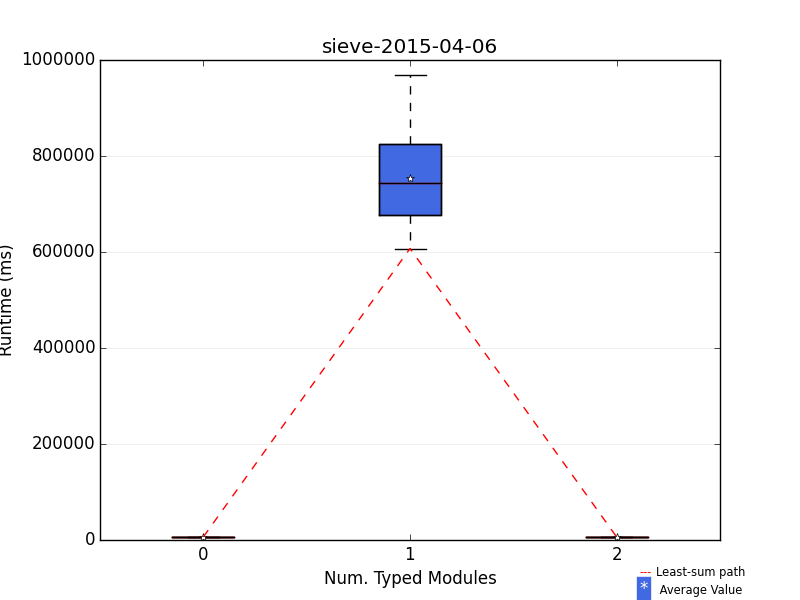
\includegraphics[width=\textwidth]{boxplots/sieve-2015-04-06-boxplot.png}
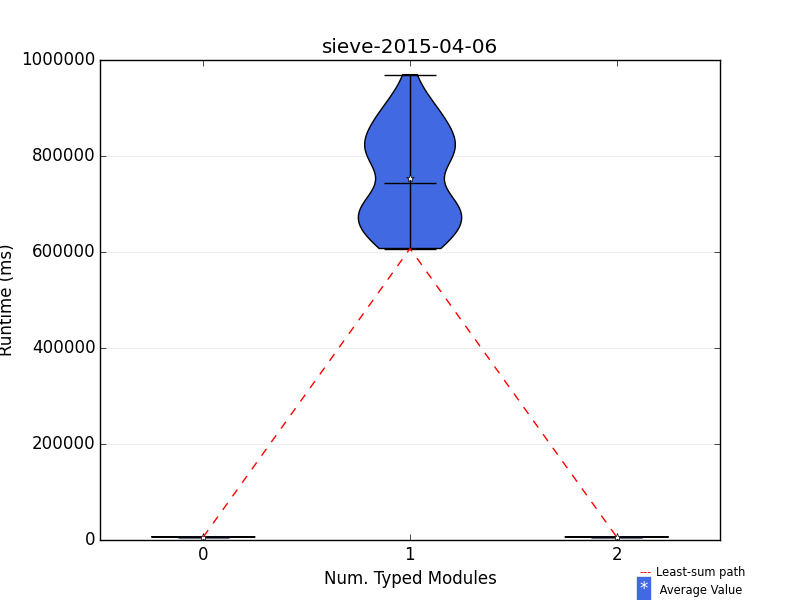
\includegraphics[width=\textwidth]{violins/sieve-2015-04-06-violin.png}
\newpage
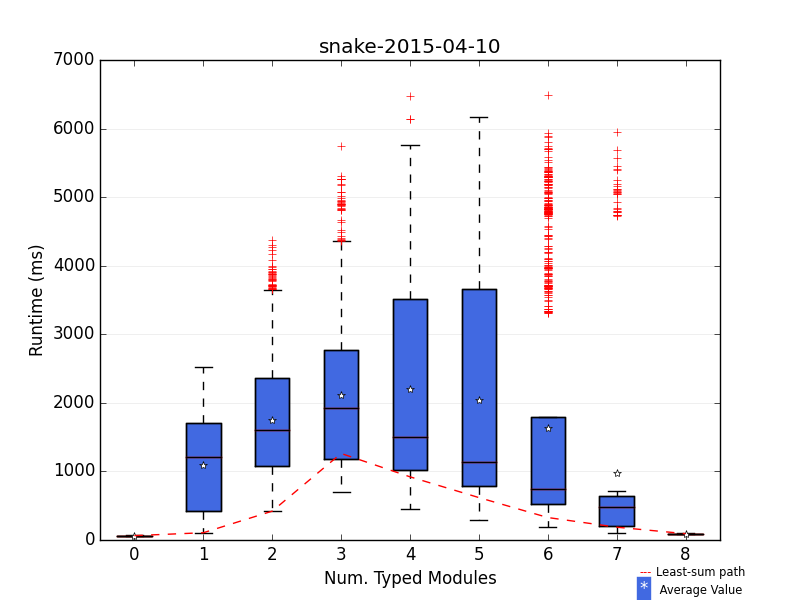
\includegraphics[width=\textwidth]{boxplots/snake-2015-04-10-boxplot.png}
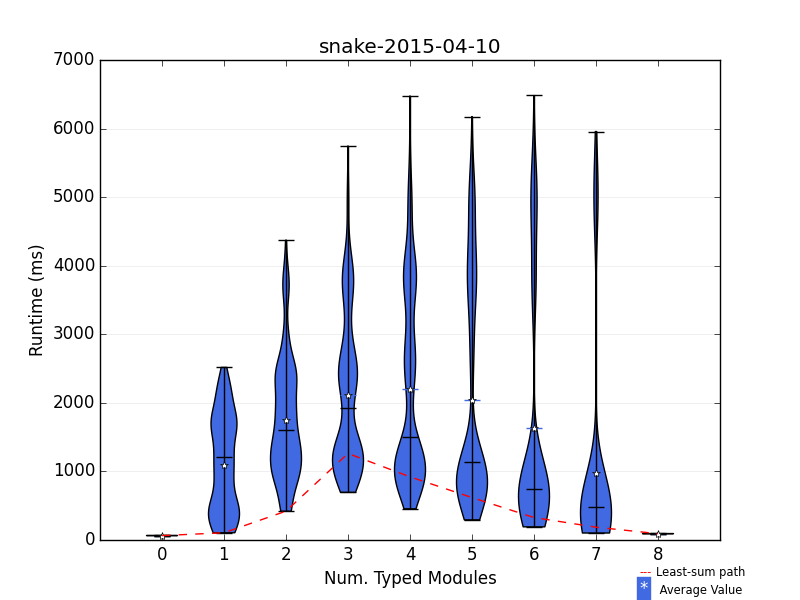
\includegraphics[width=\textwidth]{violins/snake-2015-04-10-violin.png}
\newpage
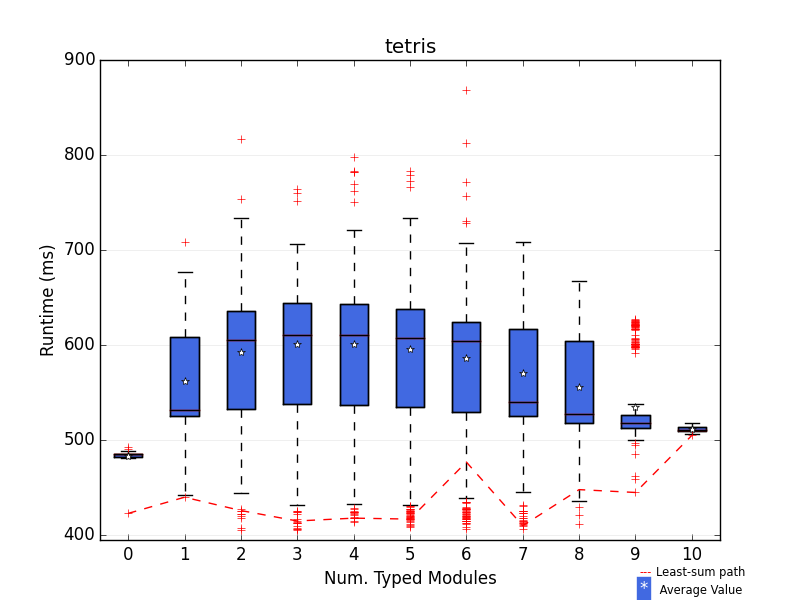
\includegraphics[width=\textwidth]{boxplots/tetris-boxplot.png}
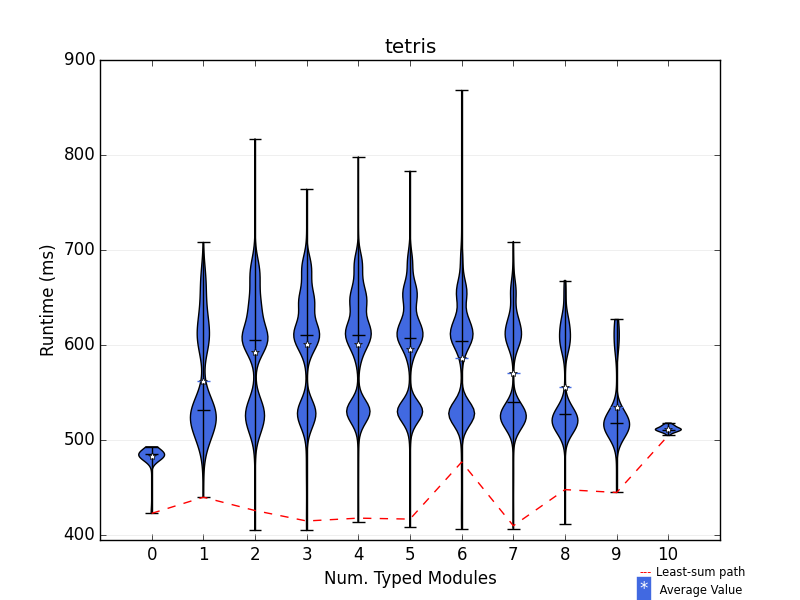
\includegraphics[width=\textwidth]{violins/tetris-violin.png}
\newpage
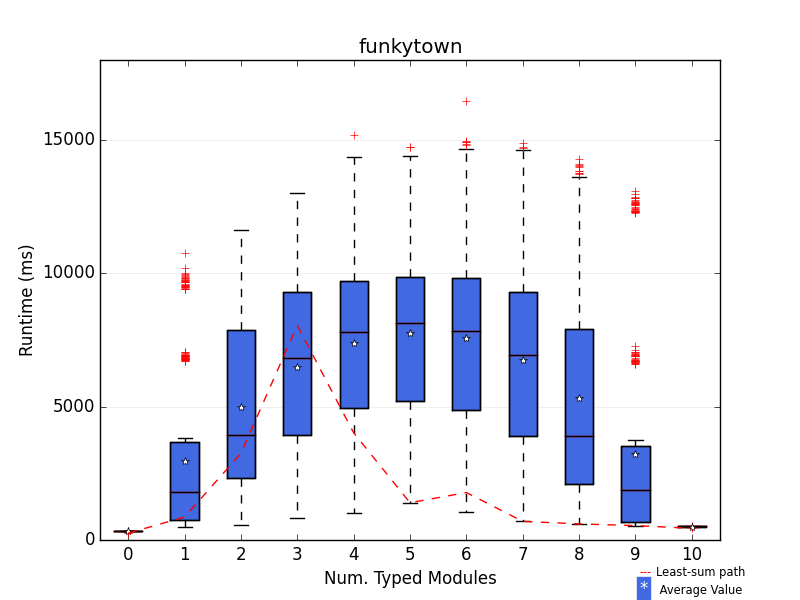
\includegraphics[width=\textwidth]{boxplots/funkytown-boxplot.png}
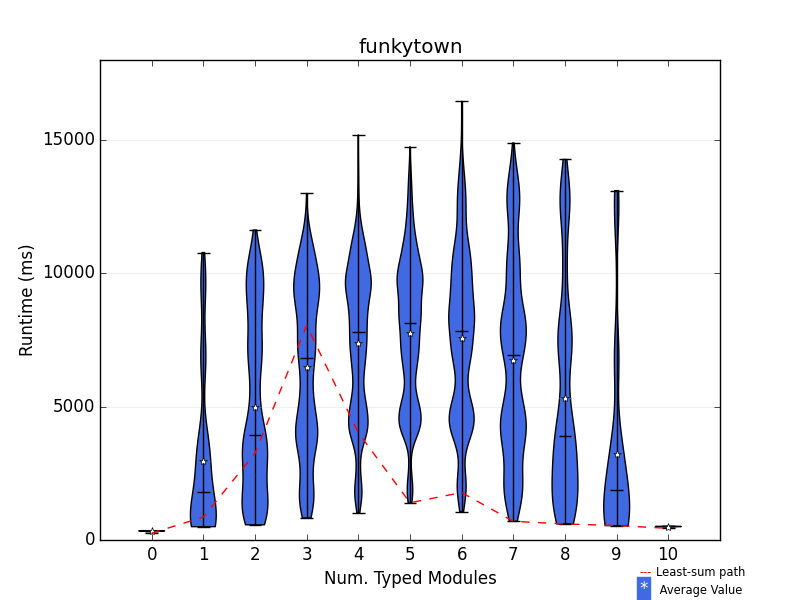
\includegraphics[width=\textwidth]{violins/funkytown-violin.png}
\newpage
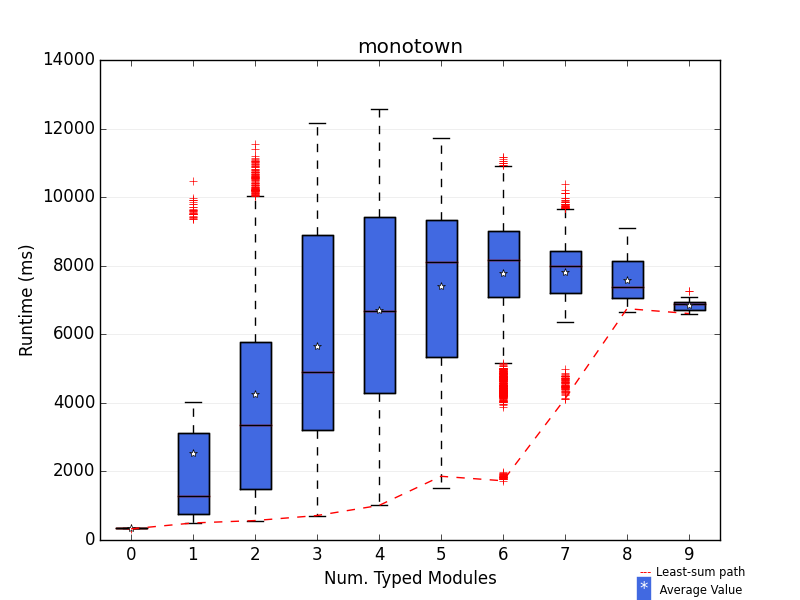
\includegraphics[width=\textwidth]{boxplots/monotown-boxplot.png}
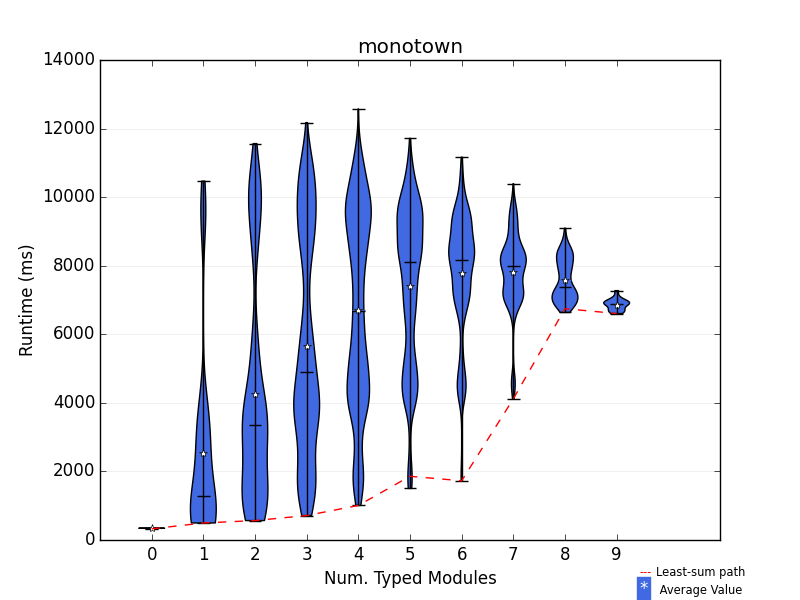
\includegraphics[width=\textwidth]{violins/monotown-violin.png}
\newpage
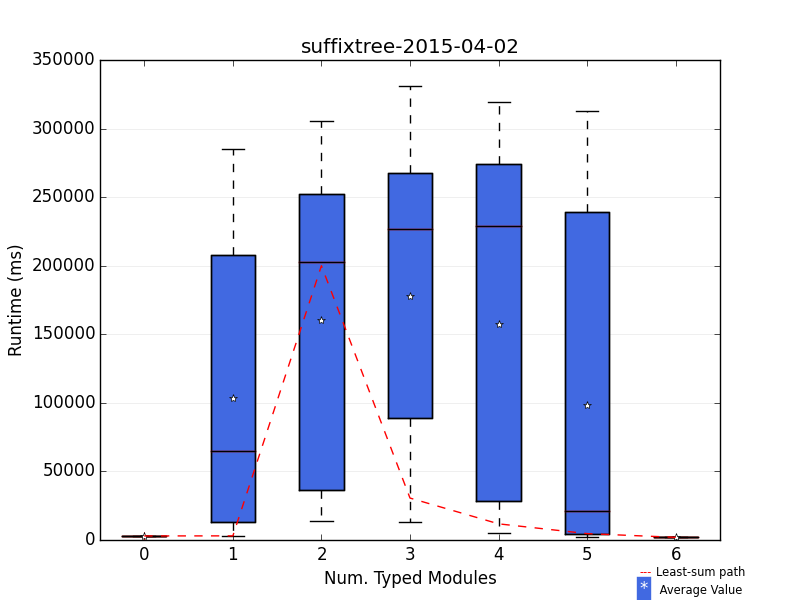
\includegraphics[width=\textwidth]{boxplots/suffixtree-2015-04-02-boxplot.png}
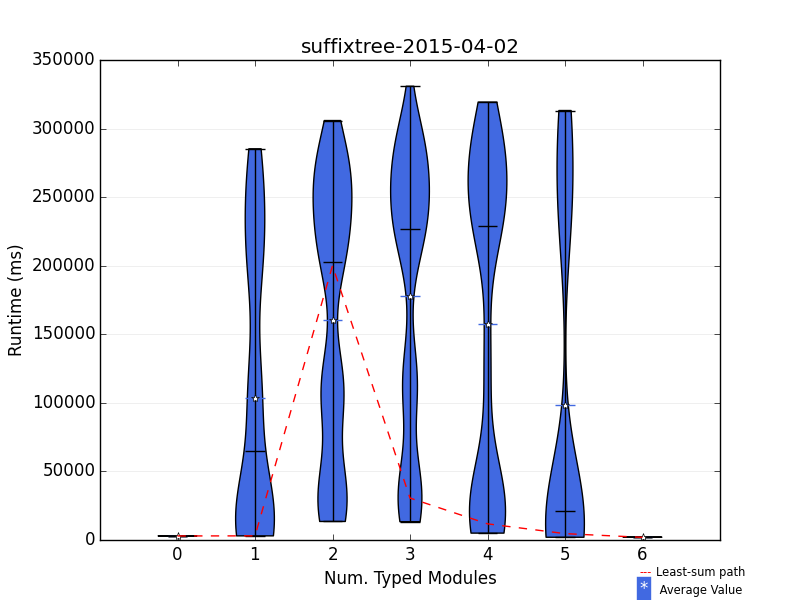
\includegraphics[width=\textwidth]{violins/suffixtree-2015-04-02-violin.png}
\newpage
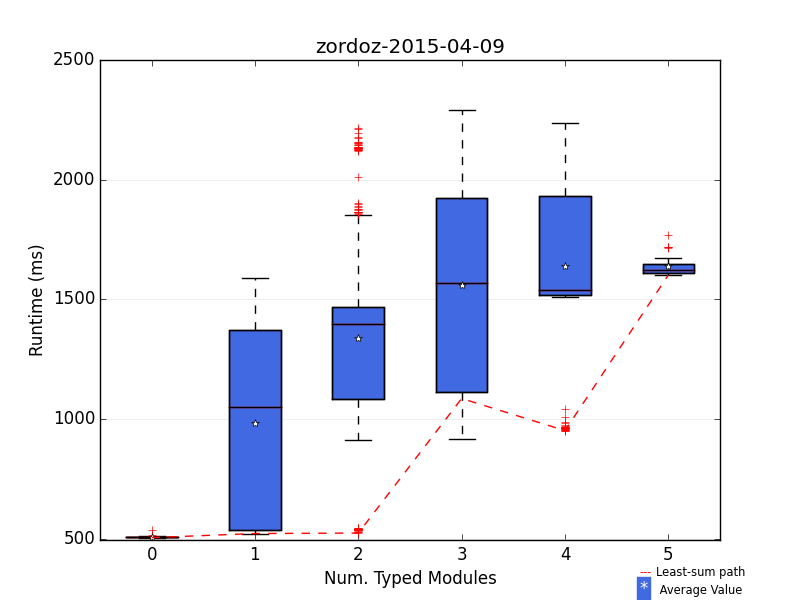
\includegraphics[width=\textwidth]{boxplots/zordoz-2015-04-09-boxplot.png}
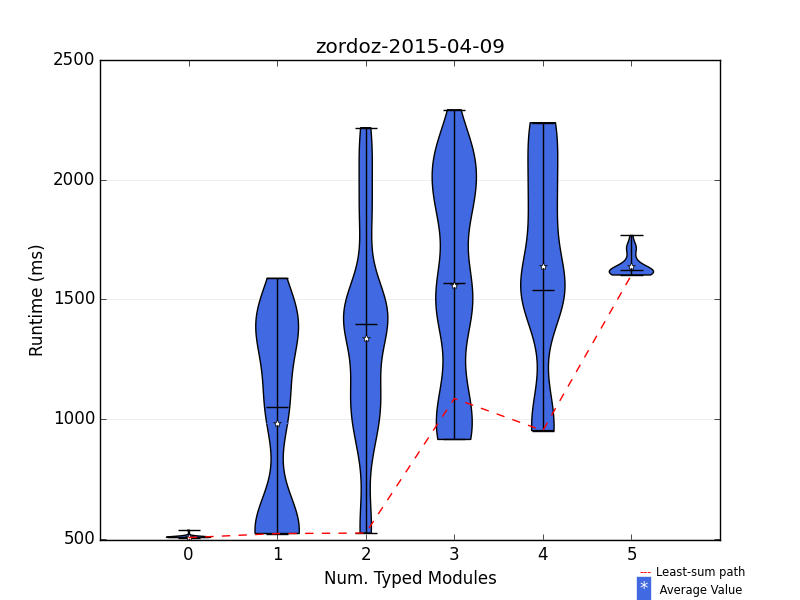
\includegraphics[width=\textwidth]{violins/zordoz-2015-04-09-violin.png}
\newpage
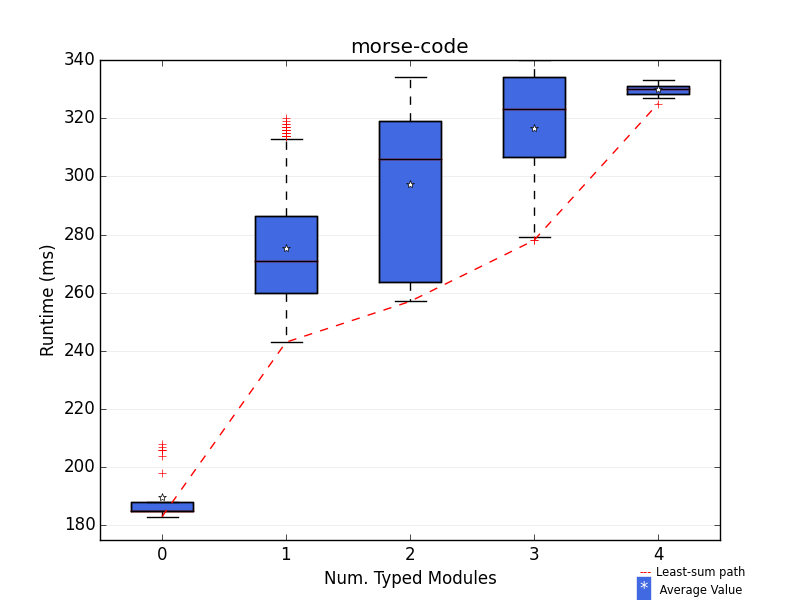
\includegraphics[width=\textwidth]{boxplots/morse-code-boxplot.png}
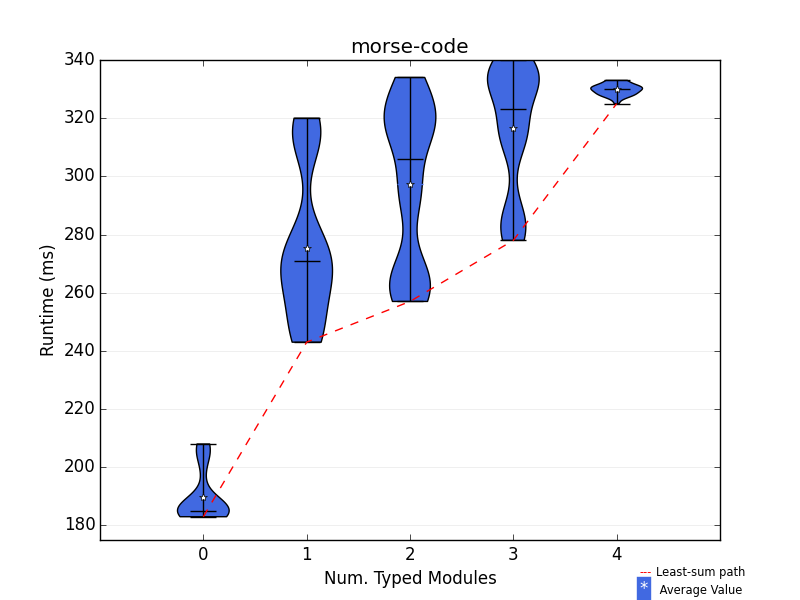
\includegraphics[width=\textwidth]{violins/morse-code-violin.png}
\newpage
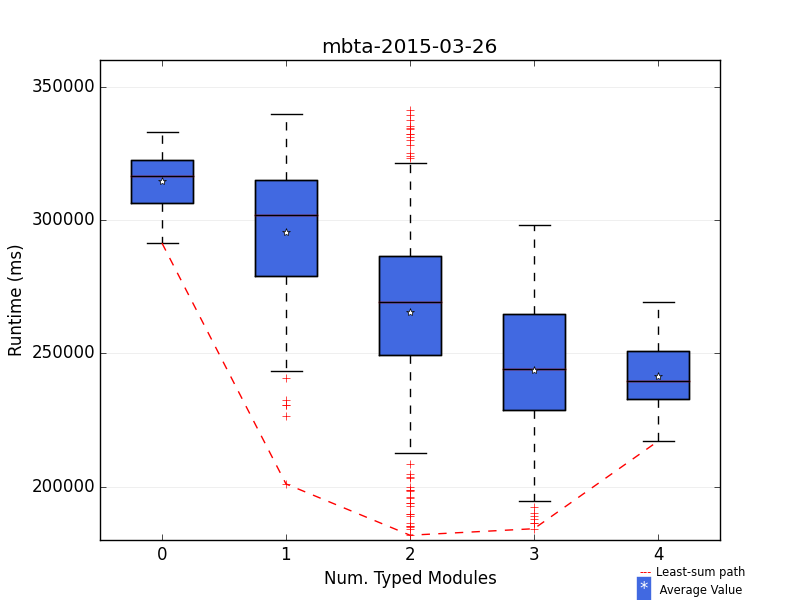
\includegraphics[width=\textwidth]{boxplots/mbta-2015-03-26-boxplot.png}
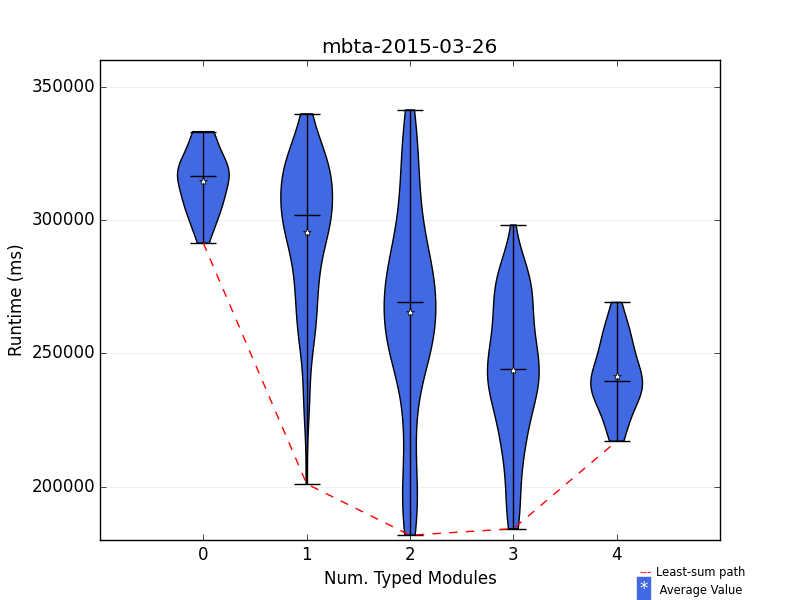
\includegraphics[width=\textwidth]{violins/mbta-2015-03-26-violin.png}
\newpage


\section{Sampling}
We claimed that the rough idea from a boxplot could be captured via simple random sampling over a small constant number of configurations, rather than running the entire lattice.
To demonstrate, we give simulated boxplots for funkytown and tetris; the two projects with at least 10 modules.

\subsection{Methodology}
Extremely simple:
\begin{itemize}
\item
  Goal: produce 10 ``boxplots''.
  So first of all, we partition the dataset into 10 parts based on the number of typed modules in a configuration.
\item
  For each partition (henceforth ``level'', as in ``level of typed-ness''), we pick 10 sample configurations.
  A configuration is a bitstring, like ``0100'' (which happens to be at ``level 1'').
  We chose 10 by the formula \texttt{(define num\_samples (max num\_modules 30))}
\item
  Each ``sample'' is, for now, a query to the pre-computed data.
  We find the matching row in the spreadsheet and take the average.
  (Really we should run that configuration \texttt{X} times and take that average.)
\item
  After sampling, we plot the sample mean and a 95\% confidence interval.
  We obtain the confidence interval using the t-test for \texttt{num\_modules - 1} degrees of freedom.
\end{itemize}

The results are quite nice, and promising.
As we scale to 20, 50, or 1000 configurations we can probably get away with taking a linear number of samples instead of an exponential number.

Note that the first box plot in each result is the ground truth data, duplicated from the above gallery.

\newpage
\subsection{Results}
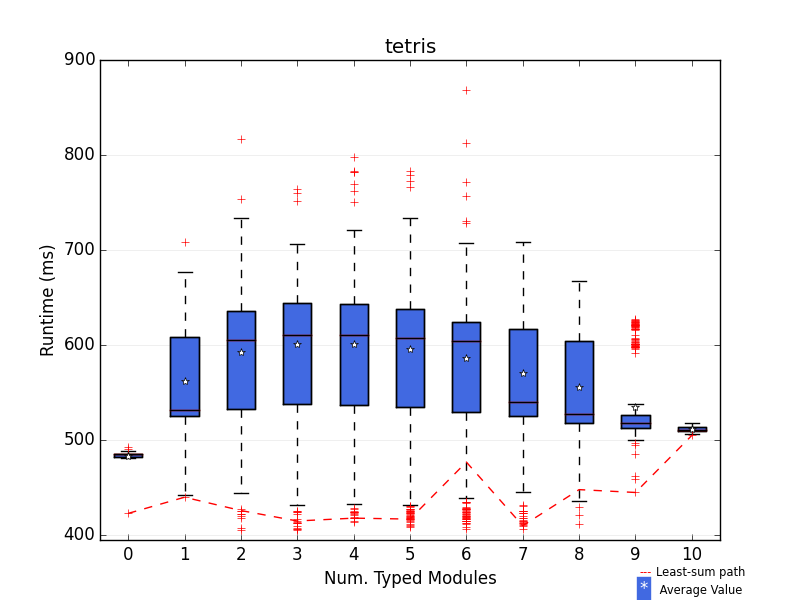
\includegraphics[width=\textwidth]{boxplots/tetris-boxplot.png}
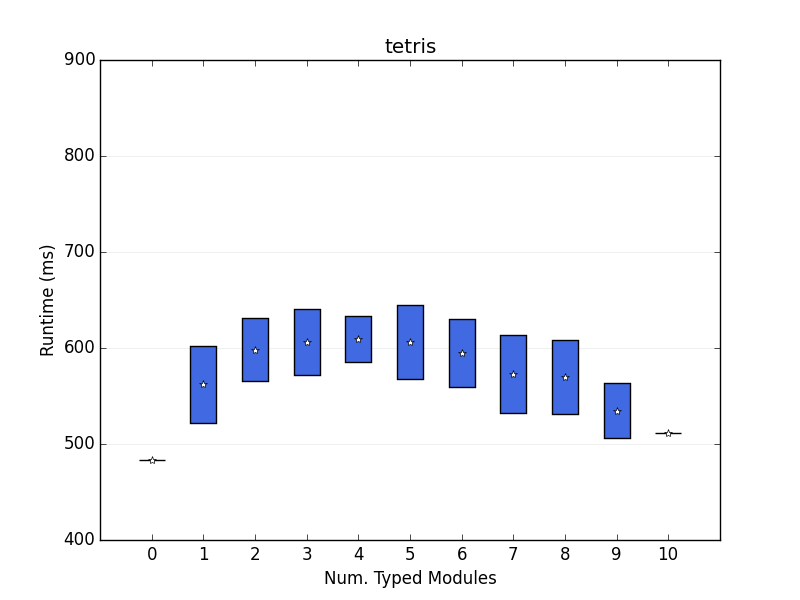
\includegraphics[width=\textwidth]{sampling/tetris-sampling-10.png}
\newpage
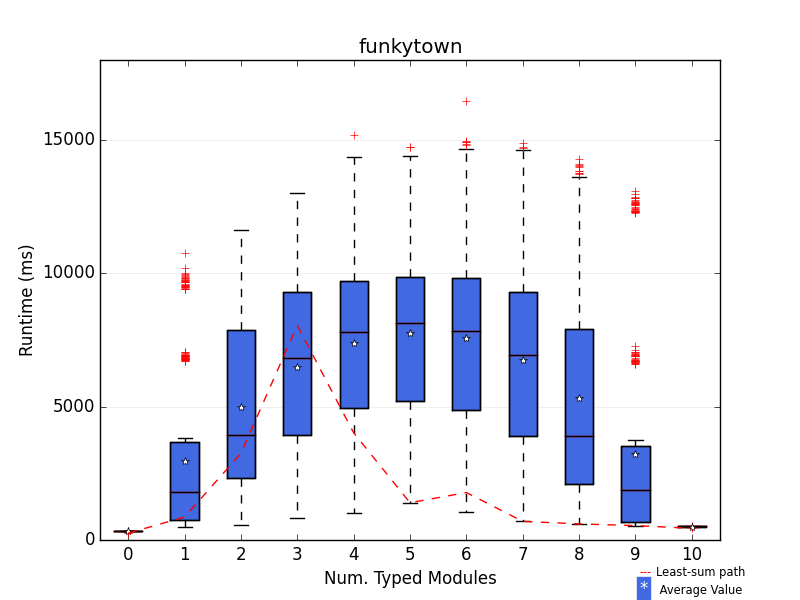
\includegraphics[width=\textwidth]{boxplots/funkytown-boxplot.png}
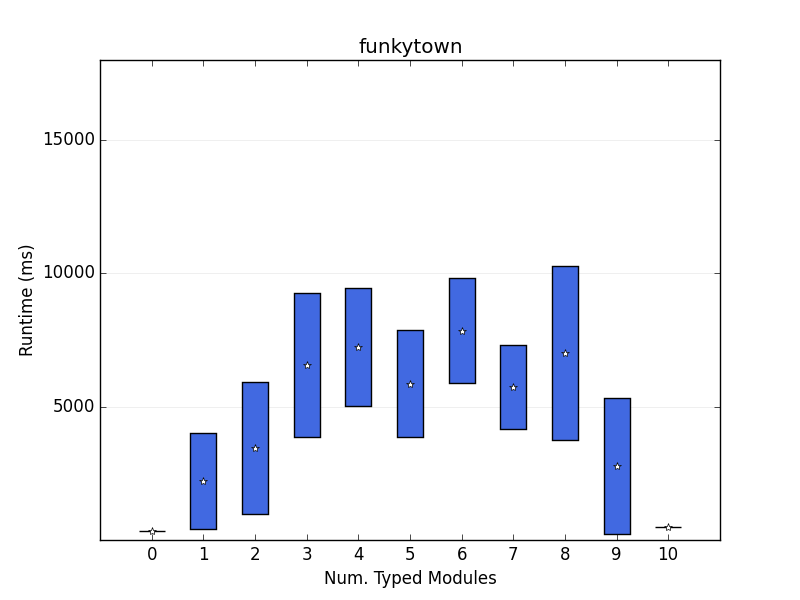
\includegraphics[width=\textwidth]{sampling/funkytown-sampling-10.png}

\newpage
\section{Big Picture}
Wondering what all runtimes look like, in perpsective?
Look no further.

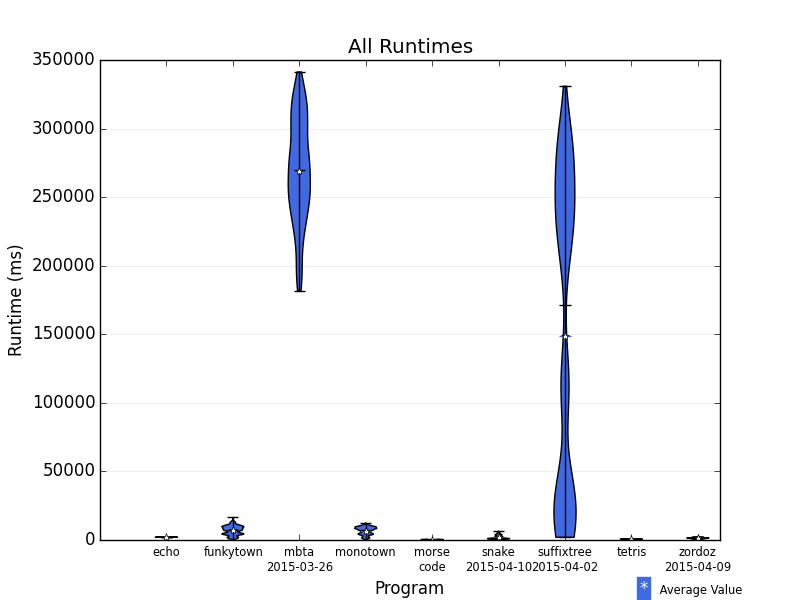
\includegraphics[width=\textwidth]{all-runtimes.png}

We should consider adjusting the running times of our benchmarks to make this picture nicer.

\newpage
\section{The Future}
Yet-unsolved problems, mostly related to getting results for projects we cannot hope to run.


\subsection{Cost of Generating Configurations}
We advocate sampling to avoid running all the configurations monolithically, but there is another cost.
Actually adding the types to generate each configuration is difficult.
In the macro world things are not so hard, but still took a bit of work.

Simple random sampling does not address this cost of ``I cannot generate all configurations''.
On the first sample it does offer a small worklist\textemdash just add types for these \texttt{N} configurations and we're good\textemdash but re-running the experiment will ask for more and more typed configurations.

There may be research on blind or non-probabilistic sampling where the sampling function is partial over the input population.
Maybe that's a heavier solution than we need, but could be useful for the micro world.


\subsection{Learning the Distribution}
Simple random sampling tells us about what we've seen, but does not say much about the underlying distribution.
That's bad.
The underlying distribution is very interesting; even learning whether or not it is uniform would be very helpful.

For this, we plan to check what the \href{http://theory.stanford.edu/~valiant/papers/instanceOptFull.pdf}{Super Valiant Bros.} have been up to.

\end{document}
